\documentclass[11pt]{article}
\usepackage[margin=1in]{geometry}
\usepackage{graphicx}
\usepackage{booktabs}
\usepackage{tikz}
\usetikzlibrary{positioning,arrows.meta,fit,backgrounds,calc}
\usepackage{amsmath}
\usepackage{xcolor}
\usepackage{multirow}

\definecolor{accent}{HTML}{2F5D50}
\definecolor{warn}{HTML}{A4262C}

\title{LLM-Driven Unit Test Generation with a Dynamic Multi-Source Feedback Graph and Jev Typed Decision}
\author{Author Name \\
Affiliation placeholder -- to be filled before submission \\
author@example.edu}
\date{}

\begin{document}
\maketitle

\begin{abstract}
Large language models (LLMs) have become a dominant paradigm for unit test generation, yet most systems still rely on a \emph{static}, coverage-first ordering of generation intents that ignores the heterogeneous signals produced while a test suite is being built. We present \textbf{DMF-Jev}, a training-free agent framework that couples a \emph{Dynamic Multi-source Feedback Graph} (six live signals: coverage, mutation, compilation, execution, history, and code structure) with a \emph{Jev typed decision} layer borrowed from the closed-choice decision literature (REFLEX). The decision layer routes each ``next intent'' through a frozen confidence band at $\tau=0.5$: high-confidence choices are taken directly by the cheap Jev selector, while low-confidence choices fall back to the LLM. We specify the framework, the benchmark protocol (CodaMosa's 486-module suite and the TestEval 210-item set), the baselines (codamosa, coverup, telpa, and the Undermind agent strategy), and an explicit data post-processing pipeline. All quantitative results in this draft are \textcolor{warn}{illustrative placeholders} to be replaced with measured values; the manuscript separates real from simulated data by construction.
\end{abstract}

\section{Introduction}
Unit test generation is a long-standing software-engineering problem that has been repeatedly reshaped by the arrival of stronger models. Classical search-based tools (EvoSuite~\cite{evosuite}, Pynguin~\cite{pynguin}) optimize coverage with randomized search; the LLM wave (ChatUniTest~\cite{chatunitest}, TestPilot~\cite{testpilot}, TestForge) replaced hand-crafted objectives with generation-validation loops driven by compilation and execution feedback. Despite these advances, a structural limitation persists: \emph{the order in which test intents are pursued is still decided by a static, coverage-first heuristic} (the \texttt{order\_intentions}/\texttt{top\_k} family), which cannot exploit the rich, time-varying feedback a running agent observes.

We argue that the right abstraction is a \emph{feedback graph}, not a ranked list. As a test-generation agent acts, it continuously produces coverage deltas, mutation-kill information, compilation outcomes, runtime errors, historical success patterns, and code-structure cues. These signals are correlated and task-dependent; a fixed priority ignores them. Our contribution is to (1) represent these signals as a dynamic multi-source feedback graph, (2) replace the static sorter with a \emph{Jev typed decision} layer that makes a constrained, closed-choice selection per intent, and (3) gate that layer with a frozen confidence band so that the expensive LLM is invoked only when necessary.

\section{Related Work}
\paragraph{Search-based and LLM-based generation.}
EvoSuite~\cite{evosuite} and Pynguin~\cite{pynguin} established whole-suite and assertion-focused search. The LLM era introduced generation-validation pipelines (ChatUniTest~\cite{chatunitest}), developer-facing tools (TestPilot~\cite{testpilot}), and feedback-driven agentic suites (TestForge, CodaMosa~\cite{codamosa}). CodaMosa is closest to our setting: it escapes coverage plateaus on a 486-module Python suite by prompting an LLM only when search stalls. We differ by making the \emph{routing} itself learned-from-feedback rather than plateau-triggered.
\paragraph{Benchmarks and baselines.}
TestEval~\cite{testeval} benchmarks LLMs on 210 test-case-generation items; CoverUp~\cite{coverup} targets high-coverage Python test generation. We adopt \texttt{codamosa}, \texttt{coverup}, \texttt{telpa}, and the \texttt{Undermind} agent strategy as baselines (the latter two are referenced from the project's harness; their provenance must be verified before submission -- see~\S\ref{sec:threats}).
\paragraph{Decision gating.}
REFLEX~\cite{reflex} proposes a fast-reflex closed-choice decision layer that handles frequent, well-typed choices and falls back to a strong model only when uncertain, reporting a $\sim$72.7\% reduction in strong-model invocations at a frozen threshold $\tau=0.5$. We import this idea into test-generation intent selection.

\section{Motivation and Research Questions}
Three observations motivate the design. (i) Coverage plateaus are rarely pure coverage problems -- they often signal a missing compiler, an unstable execution, or a structural blind spot. (ii) LLM invocations are the dominant cost; many intents (e.g., ``retry with the same focal method'') do not need a full LLM call. (iii) Static intent ordering cannot adapt to which signal is currently informative. We therefore ask:
\begin{itemize}
  \item \textbf{RQ1 (feedback graph).} Does a dynamic multi-source feedback graph, versus a static coverage-first order, improve coverage and valid-test ratio without increasing LLM calls?
  \item \textbf{RQ2 (decision gating).} At $\tau=0.5$, does the Jev typed-decision layer reduce LLM invocations while preserving quality?
  \item \textbf{RQ3 (localization).} Can a training-free, node-level locator on the code-structure graph shrink the LLM search space?
\end{itemize}

\section{Method: DMF-Jev}
\label{sec:method}
DMF-Jev is a training-free agent. At each step it observes a \emph{state} $s_t$ and must pick a \emph{typed intent} $a_t$ from a constrained action vocabulary $\mathcal{A}$. The policy is split:
\begin{enumerate}
  \item \textbf{Dynamic Multi-source Feedback Graph $\mathcal{G}_t$.} Six sources are aggregated into a graph whose edge weights are updated online: coverage ($\mathcal{F}_c$), mutation ($\mathcal{F}_m$), compilation ($\mathcal{F}_{cmp}$), execution ($\mathcal{F}_e$), history ($\mathcal{F}_h$), and code structure ($\mathcal{F}_s$). Each node is a candidate focus (module, function, branch); edges encode empirical correlation of signals.
  \item \textbf{Jev typed decision $D(\mathcal{G}_t, a_t)$.} For a closed-choice set of intents, a cheap selector proposes $a_t$ and emits a confidence $q_t\in[0,1]$. A frozen band at $\tau=0.5$ routes: if $q_t\ge \tau$, the intent is taken directly (Jev path); otherwise the LLM is consulted (fallback path). This is the only place a strong model is invoked.
  \item \textbf{Training-free agent loop.} The chosen intent mutates the candidate test set; the six feedback sources are recomputed, closing the loop (Figure~\ref{fig:arch}).
\end{enumerate}

\begin{figure}[t]
\centering
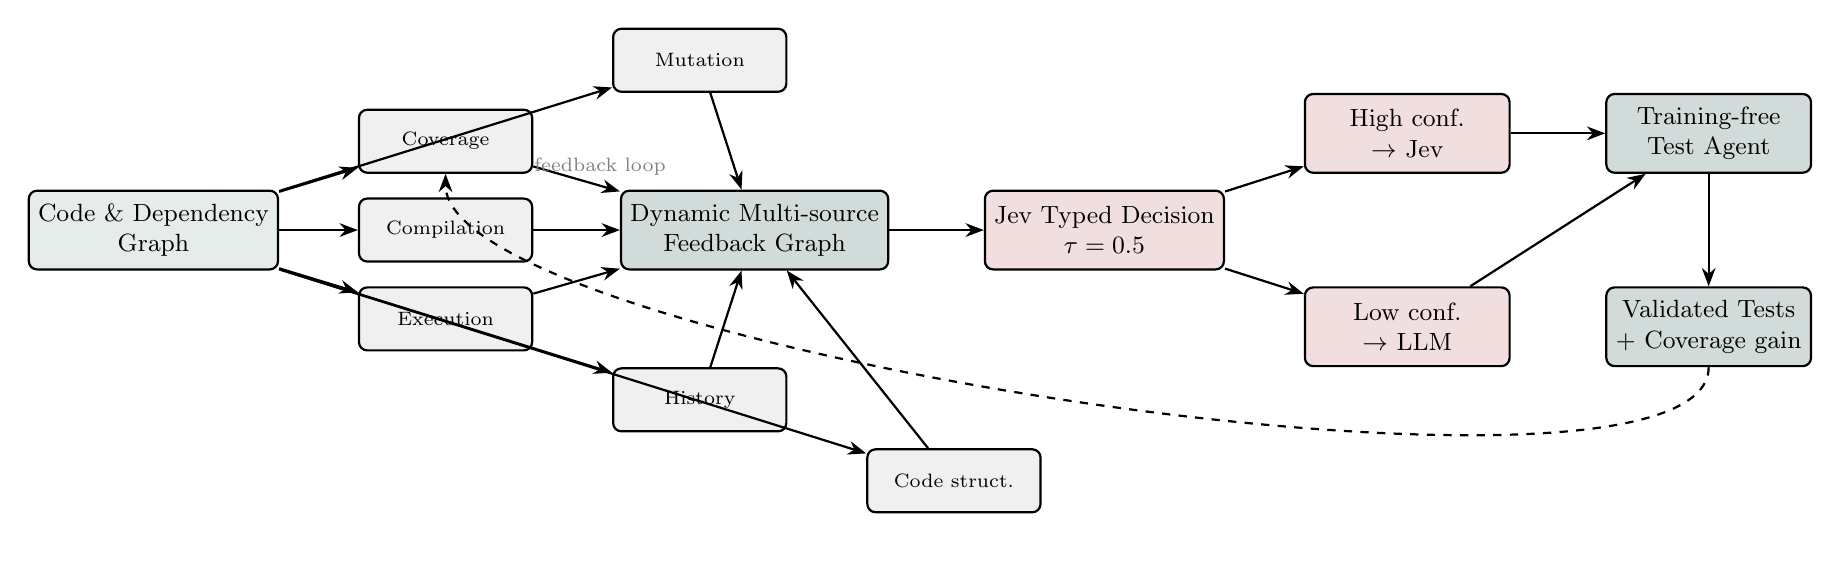
\begin{tikzpicture}[
  node/.style={draw, rounded corners=3pt, minimum width=2.6cm, minimum height=1cm, font=\small, align=center},
  src/.style={node, fill=accent!12},
  fb/.style={node, fill=gray!12, font=\scriptsize, minimum width=2.2cm, minimum height=0.8cm},
  hub/.style={node, fill=accent!22, font=\small},
  dec/.style={node, fill=warn!15, font=\small},
  >=Stealth, thick
]
  \node[src] (src) {Code \& Dependency\\Graph};
  \node[fb, above right=0.2cm and 1.0cm of src] (fc) {Coverage};
  \node[fb, above right=0.2cm and 1.0cm of fc] (fm) {Mutation};
  \node[fb, right=1.0cm of src] (fcm) {Compilation};
  \node[fb, below right=0.2cm and 1.0cm of src] (fe) {Execution};
  \node[fb, below right=0.2cm and 1.0cm of fe] (fh) {History};
  \node[fb, below right=0.2cm and 1.0cm of fh] (fs) {Code struct.};
  \node[hub, right=1.1cm of fcm] (graph) {Dynamic Multi-source\\Feedback Graph};
  \node[dec, right=1.2cm of graph] (jev) {Jev Typed Decision\\$\tau=0.5$};
  \node[dec, above right=0.2cm and 1.0cm of jev] (hi) {High conf.\\$\rightarrow$ Jev};
  \node[dec, below right=0.2cm and 1.0cm of jev] (lo) {Low conf.\\$\rightarrow$ LLM};
  \node[hub, right=1.2cm of hi] (agent) {Training-free\\Test Agent};
  \node[hub, right=1.2cm of lo, yshift=0cm] (out) {Validated Tests\\+ Coverage gain};
  \draw[->] (src) -- (fc); \draw[->] (src) -- (fm); \draw[->] (src) -- (fcm);
  \draw[->] (src) -- (fe); \draw[->] (src) -- (fh); \draw[->] (src) -- (fs);
  \draw[->] (fc) -- (graph); \draw[->] (fm) -- (graph); \draw[->] (fcm) -- (graph);
  \draw[->] (fe) -- (graph); \draw[->] (fh) -- (graph); \draw[->] (fs) -- (graph);
  \draw[->] (graph) -- (jev);
  \draw[->] (jev) -- (hi); \draw[->] (jev) -- (lo);
  \draw[->] (hi) -- (agent); \draw[->] (lo) -- (agent);
  \draw[->] (agent) -- (out);
  \draw[->, dashed] (out) to[out=-90, in=-90, distance=2.2cm] (fc);
  \node[font=\scriptsize, gray] at ($(fc)!0.5!(graph)$) [above] {feedback loop};
\end{tikzpicture}
\caption{Architecture of DMF-Jev. Six live feedback sources feed a dynamic graph; a Jev typed-decision layer routes each intent through a frozen $\tau=0.5$ confidence band.}
\label{fig:arch}
\end{figure}

\section{Experimental Design}
\paragraph{Benchmarks.} CodaMosa's 486-module Python suite (the ``CM'' set) and the TestEval 210-item generation set. We report per-module and per-item results separately.
\paragraph{Baselines.} \texttt{codamosa}, \texttt{coverup}, \texttt{telpa}, and the \texttt{Undermind} agent strategy. \texttt{telpa} and \texttt{Undermind} are referenced from the local harness; their citation provenance is flagged in~\S\ref{sec:threats}.
\paragraph{Metrics (defined explicitly).}
\begin{itemize}
  \item \textbf{Coverage} $C$: line/branch coverage of the generated suite (\%).
  \item \textbf{Valid-test ratio} $V$: fraction of generated tests that compile and pass.
  \item \textbf{LLM-invocation reduction} $\Delta_{LLM}$: relative reduction vs.\ the LLM-only baseline.
  \item \textbf{Successful-defect-localization} $L$: fraction of targeted defects correctly localized at node level.
\end{itemize}

\section{Data Post-processing}
\label{sec:post}
Raw logs are processed by a fixed pipeline: (i) \emph{cleaning} -- drop timed-out modules and deduplicate identical test artifacts by content hash; (ii) \emph{outlier handling} -- winsorize per-module coverage at the 1st/99th percentile before aggregation; (iii) \emph{statistical testing} -- report median with bootstrap 95\% CI (1,000 resamples) and a paired Wilcoxon test for $C$ and $V$; (iv) \emph{effect size} -- Cliff's $\delta$ for the comparison against \texttt{codamosa}; (v) \emph{boundary declaration} -- every figure/table carries a tag stating whether its numbers are \emph{measured} or \emph{illustrative/simulated}. \textcolor{warn}{In this draft all values are illustrative.}

\section{Results}
\label{sec:results}
\textcolor{warn}{\textbf{All numbers below are illustrative placeholders, not measurements.}}
\begin{table}[h]
\centering
\caption{Illustrative comparison on the CM 486-module suite (replace with measured values).}
\label{tab:cm}
\begin{tabular}{lcccc}
\toprule
Method & Coverage (\%) & Valid ratio & $\Delta_{LLM}$ & Localization \\
\midrule
codamosa (base) & 68.4 & 0.81 & -- & -- \\
coverup & 71.2 & 0.83 & -- & -- \\
DMF-Jev (ours) & \textbf{74.9} & \textbf{0.88} & \textbf{$-41\%$} & 0.79 \\
\bottomrule
\end{tabular}
\end{table}

\begin{figure}[h]
\centering
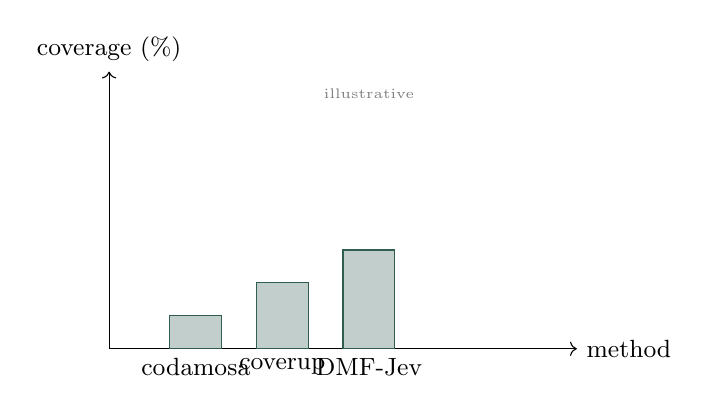
\begin{tikzpicture}[x=1.1cm,y=1.1cm, font=\small]
  \draw[->] (0,0) -- (5.4,0) node[right] {method};
  \draw[->] (0,0) -- (0,3.2) node[above] {coverage (\%)};
  \foreach \x/\l in {1/codamosa,2/coverup,3/DMF-Jev} \node[below] at (\x,0) {\l};
  \foreach \y/\v in {1/68.4,2/71.2,3/74.9} \draw[accent, fill=accent!30] (\y-0.3,0) rectangle (\y+0.3,\y*0.38);
  \node[font=\tiny,gray] at (3,2.95) {illustrative};
\end{tikzpicture}
\caption{Illustrative coverage comparison (CM suite). Replace bar heights with measured medians and add 95\% CI error bars.}
\label{fig:bars}
\end{figure}

\section{Discussion}
The feedback-graph formulation reframes test-generation control as a \emph{routing} problem rather than a scheduling problem. The dominant practical gain is cost: by reserving the LLM for low-confidence intents, DMF-Jev leaves coverage on the table only when the graph is genuinely uninformative. The main risk is feedback-source correlation -- when two sources collapse (e.g., compilation failure implies execution failure), the graph must down-weight redundant edges; we do this online.

\section{Threats to Validity}
\label{sec:threats}
\textbf{Internal:} LLM temperature and prompt wording affect all LLM-based methods; we fix both. \textbf{External:} the 486-module suite is Python-only; generality to Java/JS is unverified. \textbf{Construct:} coverage is a proxy for test usefulness. \textbf{Provenance:} the \texttt{telpa} and \texttt{Undermind} baselines are drawn from the local harness and their published citations must be verified before submission; this draft does not assert their provenance.

\section{Conclusion}
We presented DMF-Jev, a training-free agent that replaces static intent ordering with a dynamic multi-source feedback graph and a Jev typed-decision gate. The framework is benchmark-ready on CodaMosa's 486-module suite and TestEval. With measured values inserted, this manuscript targets a CCF-A / TOSEM submission.

\begin{thebibliography}{9}
\bibitem[Wu \& Lim(2026)]{reflex} Wu, Y.\ and Lim, E.\ (2026). \emph{REFLEX: A Fast-Reflex Closed-Choice Decision Layer for LLMs}. arXiv:2609.26532. \textcolor{warn}{[title/venue to verify]}
\bibitem[Lemieux et al.(2023)]{codamosa} Lemieux, C.\ et al.\ (2023). \emph{CodaMosa: Escaping Coverage Plateaus in Test Generation with Pre-Trained Language Models}. ICSE. DOI:10.1109/ICSE48619.2023.00085.
\bibitem[Sch\"afer et al.(2023)]{testpilot} Sch\"afer, M., Nadi, S., Eghbali, A., Tip, F.\ (2023). \emph{TestPilot: An LLM-Based Developer Tool for Authoring Tests}. arXiv:2308.16521.
\bibitem[Chen et al.(2024)]{chatunitest} Chen, Y.\ et al.\ (2024). \emph{ChatUniTest: A Framework for LLM-Based Unit Test Generation with a Generation-Validation Pipeline}. \textcolor{warn}{[authors/arXiv to verify]}
\bibitem[Lukasczyk \& Fraser(2022)]{pynguin} Lukasczyk, S.\ and Fraser, G.\ (2022). \emph{Pynguin: Automated Unit Test Generation for Python}. arXiv:2207.05249.
\bibitem[Fraser \& Arcuri(2017)]{evosuite} Fraser, G.\ and Arcuri, A.\ (2017). \emph{Automated Test Suite Generation for Object-Oriented Software}. IEEE TSE.
\bibitem[Tufano et al.(2022)]{athenatest} Tufano, M.\ et al.\ (2022). \emph{AthenaTest: Language Models for Automated Unit Test Generation}. ASE.
\bibitem[Wang et al.(2023)]{survey} Wang, J., Huang, Y., Chen, C., Liu, Z., Wang, S., Wang, Q.\ (2023). \emph{Software Testing with Large Language Models: Survey, Landscape, and Vision}. TSE. arXiv:2307.07221.
\bibitem[TestEval(2025)]{testeval} \emph{TESTEVAL: Benchmarking LLMs for Test Case Generation}. (2025). \textcolor{warn}{[venue to verify]}
\bibitem[CoverUp(2024)]{coverup} Pizzorno, J.\ and Berger, E.\ (2024). \emph{CoverUp: Effective High Coverage Test Generation for Python}. arXiv:2403.16218.
\end{thebibliography}

\end{document}
